%!TEX root = ../doc.tex
\chapter{Recherche}
\label{sec:recherche}

\section{Apps}
Die Recherche im Google Play Store hat ergeben dass einige Apps existieren, welche ähnliche Funktionalität wie die in dieser Arbeit zu entwickelnde App auch anbietet. Im folgenden werden 4 Apps genauer analysiert.

\subsection{Tasker}
Tasker\citep{google.play.tasker} ist eine App welche auf den ersten Blick alles anbietet. Die App kann beinahe auf jegliche Statusänderung reagieren. Sei es GPS Koordinaten oder eine SMS mit einem bestimmten Kennwort. Es erlaubt auch das Ausführen von Aktionen beim Verbinden oder Verlassen eines Wireless LANs. Die App wirkt aber auf den ersten Blick sehr umständlich und Kostet 3.99 CHF.

\subsection{Task Center}
Task Center\citep{google.play.taskcenter} scheint der schlanke Bruder von Tasker zu sein. Die App kann gratis installiert werden und ist mit In-App Käufen auch Werbefrei. Bei Task Center wird die Aktion jedoch nur bei Veränderung des Wireless LAN Verbingunsstatus ausgeführt. Dabei spielt der Netzwerkname bzw. die SSID keine Rolle.

\subsection{NFC Actions}
NFC Actions\citep{google.play.nfcactions} hat ein sehr ähnliches Prinzip wie die zu entwickelnde App aber führt diese beim erkennen eines NFC Tags aus. Dabei können AKtionen wie Bluetooth Ein oder Ausschalten oder das anrufen einer Telefonnummer ausgeführt werden. Zusätzlich lassen sich eigene NFC Tags schreiben welche dann bestimmte Aktionen auslösen.

\subsection{Trigger}
Trigger\citep{google.play.trigger} ist die App welche dem in dieser Arbeit beschriebenen Konzept am nähsten kommt. Aktionen können beim erreichen oder Verlassen von Wireless LANs ausgeführt werden. Das gleiche gilt auch für ads erreichen von GPS Koordinaten, NFC Tags und Bluetooth Netzwerke. Die App ist sehr umfangreich und daher aber auch Fehleranfällig.

\subsection{Fazit}
Die 3 analysierten Apps sowie die anderen welche bei der Recherche zum Vorschein kamen bieten einen ähnlichen Funktionsumfang an wie die App welche im Rahmen dieser Arbeit erstellt werden soll. Jedoch zeigen alle Apps gewisse Defizite auf welche die Entwicklung einer neuen App rechtfertigen. Einige Apps sind so umfangreich dass sie nicht mehr intuitiv zu bedienen sind andere wiederum lassen nur einen sehr beschränken Auslöser zu.




\section{Android SDK}
Bei der Entwicklung soll besonders auf die Energiesparsamkeit der App geachtet werden. Das Konzept der App ist nicht neu und kann spielend einfach mit einer App, welche Aktionen beim erreichen bestimmte GPS Koordinaten ausführt, umgesetzt werden. Jedoch verbrauchen solche Apps sehr viel Energie und können daher unter Umständen am entsprechenden Ort statt der Ausgeführten Aktion nur noch einen Schwarzen Bildschirm anzeigen. Diese soll bei der Ausführung der zu entwickelnden App nicht passieren. Daher soll die App nur aktiv werden wenn das System eine änderung des Wireless LAN Status erkennt hat. Dies verhindert dass die App in regelmässigen Intervallen den Status selber überprüfen muss. Zusätzlich muss beachtet werden dass beim Erreichen bzw. Verlassen eines Wireless LANs das Mobiltelefon meist nicht aktiv im Gebrauch ist. Daher muss die Aktion im Hintergrund ausgeführt werden können. Das Android Software Developer Kit bietet dafür einige Tools und APIs zur Verfügung.

\subsection{BroadcastReceiver}
Ein BroadcastReceiver reagiert auf einen definierten Intent (Aktion) welcher vom Android System oder von anderen Applikationen abgesetzt wurde. Es lässt sich einen BroadcastReceiver erstellen welcher mit einem Filter wie \glqq android.net.conn.CONNECTIVITY\_CHANGE\grqq{} auf alle Verbindungswechsel reagieren kann. Das Auslesen der aktuellen Verbindungsinformationen wird in Abbildung \ref{fig:verbindungsinfo} dargestellt. Mit diesen Informationen lässt sich der Wechseln von Wireless LANs leicht erkennen.

\begin{figure}[ht]
\centering
\begin{subfigure}[b]{0.8\textwidth}
  \centering
  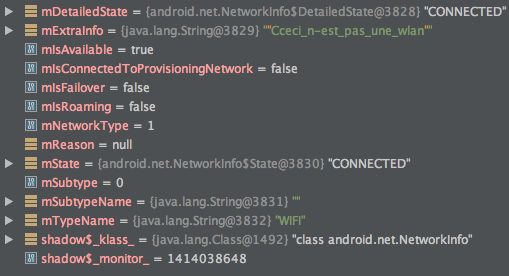
\includegraphics[width=1\linewidth]{images/debugwifi.png}
  \caption{Verbindung mit Wifi}
  \label{fig:sub1}
\end{subfigure}

\begin{subfigure}[b]{0.8\textwidth}
  \centering
  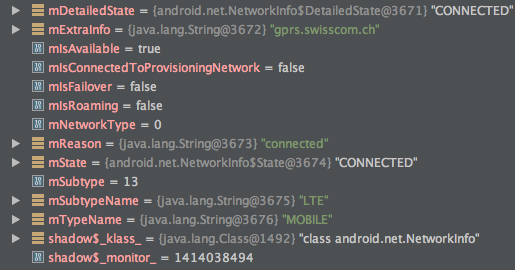
\includegraphics[width=1\linewidth]{images/debugnowifi.png}
  \caption{Verbindung ohne Wifi}
  \label{fig:sub2}
\end{subfigure}
\caption{Debug Informationen aus Android Studio}
\label{fig:verbindungsinfo}
\end{figure}


\subsection{IntentService}
Ein IntentService ist einen Android Komponente welche es erlaubt etwas in einem eigenen Thread auszuführen. Der Main Thread wird dadurch nicht gestört bzw. er wird nicht einmal benötigt, was das Ausführen bei inaktivem Mobiltelefon erlaubt. Weil der IntentService aber zur App gehört, kann auf die gemeinsamen Daten zugegriffen werden. Dadurch ist gewährleistet dass definierte Aktionen vom IntentService ausgeführt werden können.